\documentclass[a4paper,oneside,12pt]{report}
% Package yang diperlukan
\usepackage{fontspec}       % Font sistem untuk XeLaTeX/LuaLaTeX
\usepackage{setspace}       % Pengaturan jarak antarbaris
\usepackage{graphicx}      % Untuk memasukkan gambar
\usepackage{titling}       % Untuk kustomisasi halaman judul
\usepackage{geometry}      % Untuk mengatur margin halaman
\usepackage{listings}      % Untuk menampilkan blok kode
\usepackage{xcolor}        % Untuk menggunakan warna
\usepackage{float}         % Untuk kontrol penempatan float (seperti gambar)
\usepackage{hyperref}      % Untuk membuat hyperlink (URL, referensi)
\usepackage{indentfirst}   % Untuk memberi indentasi pada paragraf pertama setiap seksi
\usepackage{url}           % Untuk format URL
\usepackage{fancyhdr}      % Untuk kustomisasi header dan footer
\usepackage{tocloft}       % Untuk kustomisasi Daftar Isi
\usepackage{bookmark}      % Untuk manajemen bookmark PDF yang lebih baik

% Font dan spasi standar laporan praktikum
\setmainfont{TeX Gyre Termes}
\onehalfspacing

%======================================================================
% PENGATURAN GEOMETRI HALAMAN
%======================================================================
% Margin umum untuk isi laporan
\geometry{left=3cm, right=2.5cm, top=2cm, bottom=2.5cm}
\sloppy

%======================================================================
% PENGATURAN WARNA UNTUK BLOK KODE
%======================================================================
\definecolor{codegreen}{rgb}{0,0.6,0}
\definecolor{codegray}{rgb}{0.5,0.5,0.5}
\definecolor{codepurple}{rgb}{0.58,0,0.82}
\definecolor{backcolour}{rgb}{0.95,0.95,0.92}
\definecolor{darkblue}{rgb}{0,0,0.6}

%======================================================================
% PENGATURAN BLOK KODE (LISTINGS)
%======================================================================
% Gaya umum untuk semua blok kode
\lstdefinestyle{commonstyle}{
    backgroundcolor=\color{backcolour}, 
    breakatwhitespace=false, 
    breaklines=true, 
    captionpos=b, 
    keepspaces=true,
    numbers=left, 
    numbersep=5pt, 
    showspaces=false, 
    showstringspaces=false,
    showtabs=false, 
    tabsize=2, 
    frame=single,
    basicstyle=\ttfamily\footnotesize,
    numberstyle=\tiny\color{codegray},
    columns=flexible,
    postbreak=\mbox{\textcolor{red}{$\hookrightarrow$}\space},
    breakindent=0pt,
    breakautoindent=false
}

% Gaya khusus untuk HTML
\lstdefinestyle{htmlstyle}{
    style=commonstyle,
    language=HTML,
    commentstyle=\color{codegreen},
    keywordstyle=\color{codepurple},
    stringstyle=\color{codegreen},
    basicstyle=\ttfamily\scriptsize
}

% Gaya khusus untuk CSS
\lstdefinestyle{cssstyle}{
    style=commonstyle,
    commentstyle=\color{codegreen},
    keywordstyle=\color{darkblue},
    stringstyle=\color{codepurple},
    emph={color, background, font, margin, padding, border, display, position, width, height},
    emphstyle=\color{darkblue},
    basicstyle=\ttfamily\scriptsize
}

% Gaya khusus untuk Python
\lstdefinestyle{pythonstyle}{
    style=commonstyle,
    language=Python,
    commentstyle=\color{codegreen},
    keywordstyle=\color{darkblue},
    stringstyle=\color{codepurple},
    emph={import,from,class,def,for,while,if,else,elif,try,except,finally},
    emphstyle=\color{darkblue}
}

% Gaya khusus untuk SQL
\lstdefinestyle{sqlstyle}{
    style=commonstyle,
    language=SQL,
    commentstyle=\color{codegreen},
    keywordstyle=\color{darkblue},
    stringstyle=\color{codepurple},
    emph={SELECT,FROM,WHERE,INSERT,UPDATE,DELETE,CREATE,DROP},
    emphstyle=\color{darkblue}
}

% Gaya khusus untuk JavaScript
\lstdefinestyle{javascriptstyle}{
    style=commonstyle,
    language=JavaScript,
    commentstyle=\color{codegreen},
    keywordstyle=\color{darkblue},
    stringstyle=\color{codepurple},
    emph={function,var,let,const,return,if,for,while,do,else,switch,case},
    emphstyle=\color{darkblue}
}

%======================================================================
% PENGATURAN LAIN-LAIN
%======================================================================
% Perintah kustom untuk bingkai gambar
\newcommand{\customfbox}[1]{%
  \setlength{\fboxsep}{0pt}%
  \setlength{\fboxrule}{0.5pt}%
  \fcolorbox{black}{white}{#1}%
}

% Mengganti nama default "Figure" menjadi "Gambar"
\renewcommand{\figurename}{Gambar}
\renewcommand{\thefigure}{\arabic{figure}}

% Pengaturan Hyperlink
\hypersetup{
    colorlinks=true, 
    linkcolor=black, 
    filecolor=black, 
    urlcolor=black,
    citecolor=black,
    pdftitle={Laporan Praktikum}, 
    pdfpagemode=FullScreen, 
    breaklinks=true
}

% Pengaturan Header & Footer (nomor halaman di tengah bawah)
\pagestyle{fancy}
\fancyhf{}
\fancyfoot[C]{\thepage}
\renewcommand{\headrulewidth}{0pt}

\fancypagestyle{plain}{
    \fancyhf{}
    \fancyfoot[C]{\thepage}
    \renewcommand{\headrulewidth}{0pt}
}

%======================================================================
% PENGATURAN STRUKTUR BAB DAN DAFTAR ISI
%======================================================================
\renewcommand{\contentsname}{Daftar Isi}
\renewcommand{\bibname}{Daftar Pustaka}

% Menghilangkan nomor bab tetapi mempertahankan penomoran seksi
\renewcommand{\thechapter}{}
\renewcommand{\chaptername}{}

% Format penomoran seksi menjadi [nomor bab].[nomor seksi]
\renewcommand{\thesection}{\arabic{chapter}.\arabic{section}}
\renewcommand{\thesubsection}{\thesection.\arabic{subsection}}

\setcounter{secnumdepth}{3}
\setcounter{tocdepth}{3}

% Format Daftar Isi (TOC)
\renewcommand{\cftchapdotsep}{\cftdotsep}
\renewcommand{\cftchapleader}{\cftdotfill{\cftchapdotsep}}
\setlength{\cftchapindent}{0em}
\setlength{\cftsecindent}{2em}
\setlength{\cftsubsecindent}{4em}
\setlength{\cftchapnumwidth}{0em}
\setlength{\cftsecnumwidth}{2.5em}
\setlength{\cftsubsecnumwidth}{3.2em}
\renewcommand{\cftchappresnum}{}
\renewcommand{\cftchapaftersnum}{}

% Perintah kustom untuk membuat judul bab di TOC menjadi tebal
\newcommand{\tocboldsection}[1]{%
  \protect\renewcommand{\protect\cftchapfont}{\protect\bfseries}%
  #1%
  \protect\renewcommand{\protect\cftchapfont}{}%
}

%======================================================================
% AWAL DOKUMEN
%======================================================================
\begin{document}

% Halaman Judul
\newgeometry{left=3cm, right=2.5cm, top=2.5cm, bottom=3cm}
\begin{titlingpage}
\begin{spacing}{1}
\begin{center}
\vspace*{0.2cm}
{\large \textbf{\MakeUppercase{Laporan Praktikum}}} \\[0.4cm]
{\large \textbf{\MakeUppercase{PRAKTIKUM
PENAMBANGAN DATA}}} \\[0.4cm]
{\large \textbf{\MakeUppercase{Pertemuan 2}}} \\[0.4cm]
{\large \textbf{\MakeUppercase{EXPLORATORY DATA ANALYSIS DAN DATA PREPROCESSING}}} \\[1.5cm]


\includegraphics[height=7cm]{../template-pertemuan/images/UGM.png} \\[0.7cm]

{\normalsize \textbf{Disusun oleh:}} \\[0.4cm]
\begin{tabular}{@{}l l @{}}
  \textbf{Nama}           & : Hafidz Rizqullah Prasetya \\
  \textbf{NIM}            & : 24/535493/SV/24243 \\
  \textbf{Kelas}          & : PL5A1 \\
  \textbf{Dosen Pengampu} & : Dr. Imam Fahrurrozi, S.T., M.Cs.
\end{tabular} \\[1.2cm]

{\normalsize \textbf{PROGRAM STUDI D-IV}} \\[0.2cm]
{\normalsize \textbf{TEKNOLOGI REKAYASA PERANGKAT LUNAK}} \\[0.2cm]
{\normalsize \textbf{DEPARTEMEN TEKNIK ELEKTRO DAN INFORMATIKA}} \\[0.2cm]
{\normalsize \textbf{SEKOLAH VOKASI}} \\[0.2cm]
{\normalsize \textbf{UNIVERSITAS GADJAH MADA}} \\[0.2cm]
{\normalsize \textbf{YOGYAKARTA}} \\[0.2cm]
{\normalsize \textbf{2026}} \\[1.2cm]
\end{center}
\end{spacing}
\end{titlingpage}
\restoregeometry

\thispagestyle{empty}
\clearpage
\stepcounter{page}
\thispagestyle{empty}

% --- Daftar Isi ---
\addcontentsline{toc}{chapter}{Daftar Isi}
\tableofcontents
\clearpage

% Mengatur penomoran halaman menjadi arab dan mulai dari 3
\pagenumbering{arabic}
\setcounter{page}{3}

\chapter[Tujuan Praktikum]{Tujuan Praktikum}
\begin{enumerate}
   \item Mahasiswa mampu memahami konsep dasar Artificial Intelligence (AI) dan Machine Learning (ML).
   \item Mahasiswa mampu menerapkan Exploratory Data Analysis (EDA) untuk memahami karakteristik, distribusi, dan kualitas dataset.
   \item Mahasiswa mampu menerapkan teknik dasar data preprocessing, meliputi penanganan missing value dan duplikasi, encoding, pembagian dataset, serta scaling fitur.
\end{enumerate}
\clearpage

\chapter{Dasar Teori}

\section{Artificial Intelligence dan Machine Learning}

\subsection{Artificial Intelligence}
Artificial Intelligence (AI) adalah bidang ilmu komputer yang mengembangkan sistem
agar mampu melakukan tugas yang umumnya membutuhkan kecerdasan manusia, seperti
mengenali pola, belajar dari pengalaman, memahami informasi, dan mengambil
keputusan. Dalam penerapannya, kualitas data sangat memengaruhi kemampuan sistem
AI karena data menjadi dasar untuk menemukan pola dan menghasilkan prediksi
\cite{dicoding-workflow}.

\subsection{Machine Learning}
Machine Learning (ML) merupakan cabang AI yang memungkinkan komputer mempelajari
pola dari data dan meningkatkan kinerjanya tanpa aturan yang diprogram secara
eksplisit untuk setiap kasus. ML dapat dibagi menjadi \textit{supervised learning},
\textit{unsupervised learning}, dan \textit{reinforcement learning}. Pada
\textit{supervised learning}, data memiliki label untuk keperluan klasifikasi atau
prediksi. Pada \textit{unsupervised learning}, model mencari struktur atau pola
tersembunyi tanpa label. Sementara itu, \textit{reinforcement learning} belajar
melalui umpan balik berupa penghargaan dan hukuman
\cite{google-ml-categorical}.

\begin{figure}[H]
    \centering
    \fbox{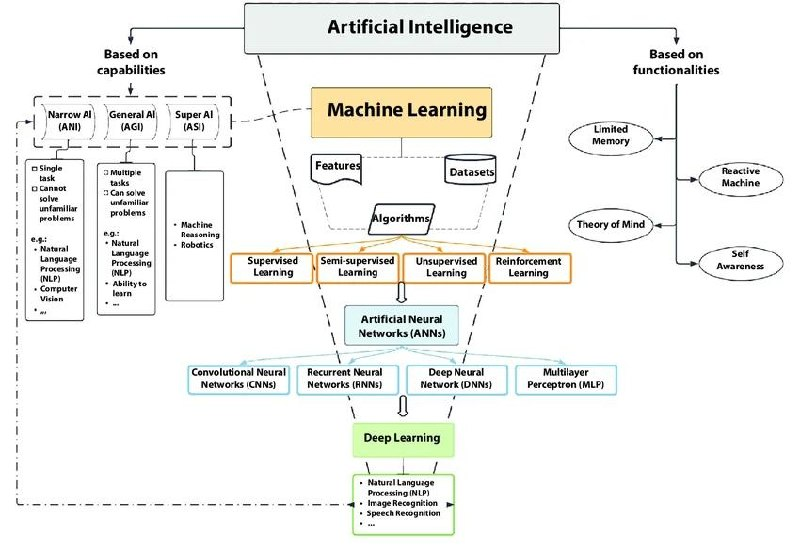
\includegraphics[width=0.85\textwidth]{images/ai-ml-relationship-diagram.jpg}}
    \caption{Klasifikasi Artificial Intelligence, Machine Learning, dan Deep Learning.}
    \label{fig:ai-ml-relationship}
\end{figure}

\section{Exploratory Data Analysis}
Exploratory Data Analysis (EDA) adalah proses memeriksa dan memahami dataset
sebelum dilakukan pemodelan. EDA digunakan untuk mengetahui struktur data, tipe
atribut, distribusi nilai, hubungan antarvariabel, outlier, missing value, dan
duplikasi. Pemeriksaan dapat dilakukan menggunakan \texttt{head()},
\texttt{tail()}, \texttt{shape}, \texttt{describe()}, dan
\texttt{isnull().sum()} pada DataFrame pandas.

Visualisasi membantu menyampaikan karakteristik data secara lebih mudah. Line
plot digunakan untuk melihat perubahan atau tren, pie chart untuk proporsi,
bar plot untuk membandingkan kategori, histogram untuk distribusi numerik,
scatter plot untuk hubungan dua variabel, box plot untuk ringkasan kuartil dan
outlier, serta violin plot untuk bentuk distribusi dan kepadatan data. Korelasi
antarvariabel numerik juga dapat dihitung dengan \texttt{corr()} untuk mengetahui
arah dan kekuatan hubungan linear \cite{ibm-eda,pandas-describe}.

\begin{figure}[H]
    \centering
    \fbox{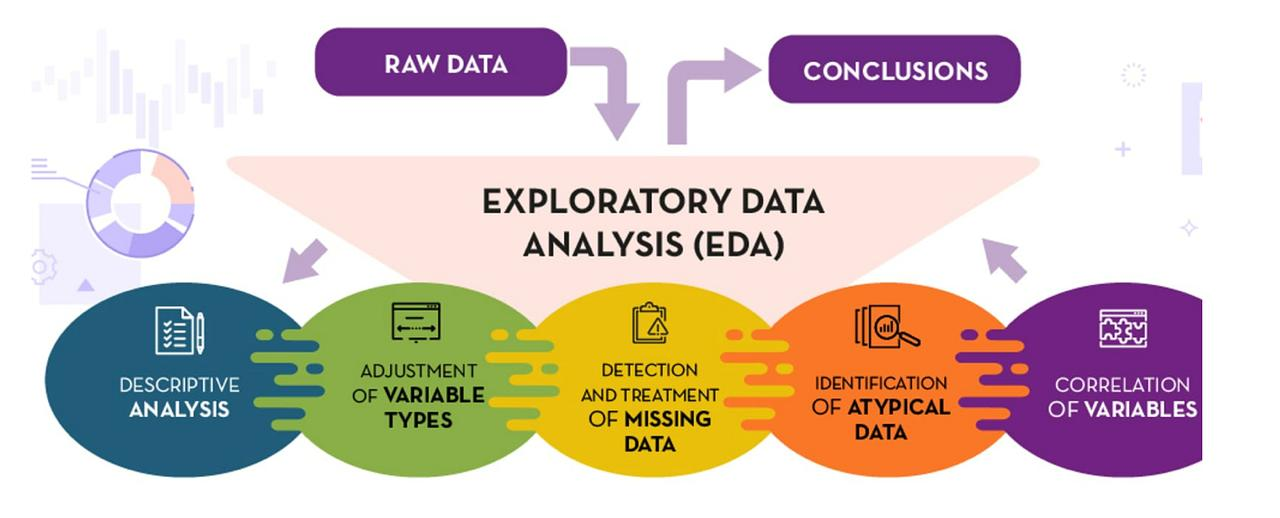
\includegraphics[width=1\textwidth]{images/eda-workflow-diagram.jpg}}
    \caption{Alur Exploratory Data Analysis mulai dari data mentah hingga menghasilkan kesimpulan.}
    \label{fig:eda-workflow}
\end{figure}

\section{Data Preprocessing}
Data preprocessing merupakan serangkaian langkah untuk membersihkan dan
mengubah data mentah menjadi data yang siap dianalisis atau digunakan oleh model
ML. Tahap ini penting karena data yang tidak konsisten, tidak lengkap, atau
memiliki skala berbeda dapat menurunkan kualitas analisis dan performa model.

\begin{figure}[H]
    \centering
    \fbox{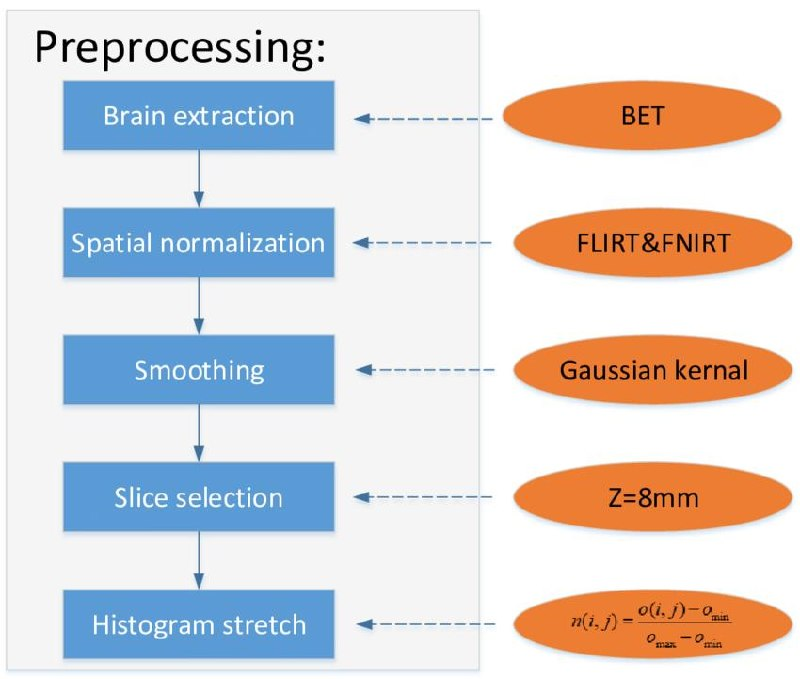
\includegraphics[width=0.82\textwidth]{images/data-preprocessing-workflow.jpg}}
    \caption{Contoh alur data preprocessing yang meliputi ekstraksi, standardisasi spasial, smoothing, pemilihan citra, dan normalisasi intensitas.}
    \label{fig:data-preprocessing-workflow}
\end{figure}

\subsection{Pembersihan Data dan Imputasi}
Missing value dapat diperiksa menggunakan \texttt{isnull().sum()}, sedangkan
baris duplikat dapat diperiksa menggunakan \texttt{duplicated().sum()}.
Missing value dapat ditangani dengan menghapus baris atau kolom yang bermasalah,
atau dengan imputasi. Nilai median sering digunakan untuk atribut numerik karena
lebih tahan terhadap outlier, sedangkan modus dapat digunakan untuk atribut
kategorikal. Duplikasi perlu dihapus apabila merepresentasikan pengamatan yang
tercatat lebih dari satu kali \cite{ilmudatapy-missing}.

\begin{figure}[H]
    \centering
    \fbox{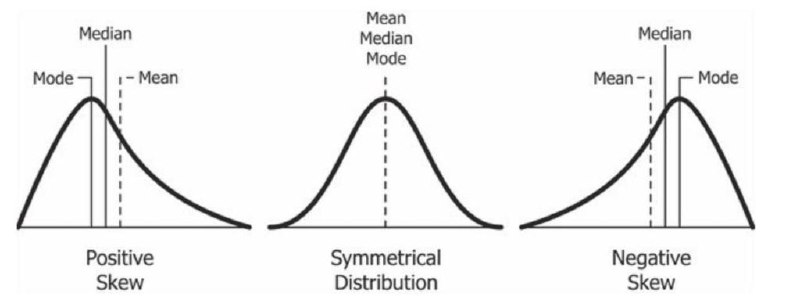
\includegraphics[width=0.9\textwidth]{images/missing-value-imputation-distributions.jpg}}
    \caption{Hubungan mean, median, dan mode pada distribusi data sebagai pertimbangan pemilihan metode imputasi.}
    \label{fig:missing-value-imputation}
\end{figure}

\subsection{Encoding Atribut Kategorikal}
Algoritma ML umumnya memerlukan input numerik. One-hot encoding mengubah kategori
menjadi beberapa kolom biner dan sesuai untuk kategori nominal. Label encoding
mengubah kategori menjadi bilangan integer dan perlu digunakan secara hati-hati
karena angka dapat dianggap memiliki urutan. Pada fitur kategorikal nominal,
one-hot encoding biasanya lebih aman untuk mencegah model menganggap adanya
hubungan ordinal yang sebenarnya tidak ada \cite{google-ml-categorical,ilmudatapy-ohe}.

\begin{figure}[H]
    \centering
    \fbox{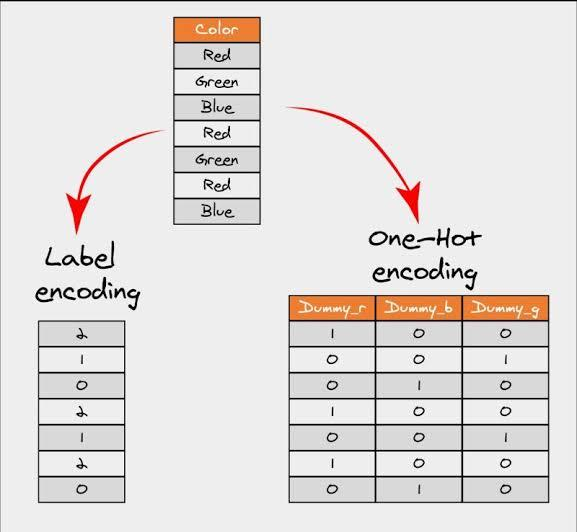
\includegraphics[width=0.72\textwidth]{images/one-hot-vs-label-encoding.jpg}}
    \caption{Perbandingan label encoding dan one-hot encoding pada variabel kategorikal.}
    \label{fig:one-hot-vs-label}
\end{figure}

\subsection{Pembagian Dataset dan Scaling}
Dataset biasanya dibagi menjadi data latih dan data uji menggunakan
\texttt{train\_test\_split()}. Data latih digunakan untuk membangun model,
sedangkan data uji digunakan untuk mengukur kemampuan generalisasi model.
Parameter pembagian harus disesuaikan dengan instruksi praktikum, misalnya
80:20.

Scaling digunakan agar fitur numerik berada pada skala yang sebanding.
\textit{Standardization} menggunakan rata-rata dan simpangan baku sehingga data
memiliki rata-rata mendekati nol dan simpangan baku mendekati satu. Sementara itu,
\textit{normalization} seperti Min-Max Scaling memetakan nilai ke rentang tertentu,
umumnya 0 sampai 1. Parameter scaler harus di-fit pada data latih saja, kemudian
digunakan untuk mentransformasi data uji agar tidak terjadi kebocoran informasi
\cite{sklearn-preprocessing,sklearn-pitfalls}.

\begin{figure}[H]
    \centering
    \fbox{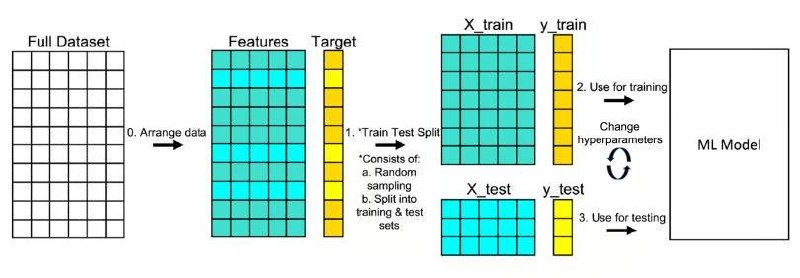
\includegraphics[width=1\textwidth]{images/train-test-split-diagram.jpg}}
    \caption{Alur pembagian features dan target menjadi data latih serta data uji menggunakan train-test split.}
    \label{fig:train-test-split}
\end{figure}

\clearpage

\chapter[\tocboldsection{Hasil dan Pembahasan}]{Hasil dan Pembahasan}

\section{Percobaan Latihan Praktikum}

Pada bagian ini saya mendokumentasikan percobaan EDA dan data preprocessing sesuai langkah pada modul Pertemuan 2. Karena screenshot hasil eksekusi belum dilampirkan, setiap lokasi keluaran notebook diberi placeholder yang akan saya ganti setelah praktikum selesai.

\subsection{Persiapan dan Impor Pustaka}
Saya menyiapkan lingkungan Python dan mengimpor pandas untuk manipulasi data, NumPy untuk komputasi numerik, Matplotlib untuk visualisasi, serta scikit-learn untuk preprocessing.

\begin{lstlisting}[style=pythonstyle,caption={Impor pustaka praktikum.}]
import pandas as pd
import numpy as np
import matplotlib.pyplot as plt
from sklearn.model_selection import train_test_split
from sklearn.preprocessing import StandardScaler, MinMaxScaler, LabelEncoder
\end{lstlisting}

\begin{figure}[H]
\centering
\fbox{\parbox[c][3cm][c]{0.9\textwidth}{\centering PLACEHOLDER\\Screenshot impor pustaka dan versi library}}
\caption{Impor pustaka yang digunakan dalam praktikum.}
\label{fig:placeholder-import}
\end{figure}

\section{Exploratory Data Analysis}
\subsection{Memuat Dataset Bank Churners}
Untuk latihan EDA, saya menggunakan dataset Bank Churners dari Kaggle. Dataset ini berisi informasi nasabah kartu kredit dengan label \texttt{Attrition\_Flag} yang menunjukkan status nasabah. Dataset saya muat menggunakan \texttt{pd.read\_csv()}.

\begin{lstlisting}[style=pythonstyle,caption={Memuat dataset Bank Churners.}]
df_churning = pd.read_csv('https://raw.githubusercontent.com/ganjar87/data_science_practice/main/BankChurners.csv')
df_churning.head()
\end{lstlisting}

\begin{figure}[H]
\centering
\fbox{\parbox[c][3cm][c]{0.9\textwidth}{\centering PLACEHOLDER\\Output df\_churning.head()}}
\caption{Lima baris pertama dataset Bank Churners.}
\label{fig:placeholder-churn-head}
\end{figure}

\subsection{Pemeriksaan dan Pemisahan Kelas}
Saya menggunakan \texttt{tail()} untuk memeriksa baris terakhir dataset. Setelah itu, saya memisahkan data menjadi nasabah aktif dan nasabah yang berhenti berdasarkan kolom \texttt{Attrition\_Flag}.

\begin{lstlisting}[style=pythonstyle,caption={Pemeriksaan akhir dan pemisahan kelas.}]
df_churning.tail()
existing_data = df_churning[df_churning['Attrition_Flag'] == 'Existing Customer']
attrited_data = df_churning[df_churning['Attrition_Flag'] == 'Attrited Customer']
\end{lstlisting}

\begin{figure}[H]
\centering
\fbox{\parbox[c][3cm][c]{0.9\textwidth}{\centering PLACEHOLDER\\Output tail() dan jumlah kelas}}
\caption{Pemeriksaan baris terakhir dan pemisahan kelas nasabah.}
\label{fig:placeholder-churn-tail}
\end{figure}

\subsection{Visualisasi Dataset Bank Churners}
Saya membuat line chart, pie chart, bar plot, dan stacked bar plot untuk melihat tren serta perbandingan kategori. Untuk data numerik, saya menggunakan histogram, scatter plot, box plot, dan violin plot. Visualisasi tersebut membantu saya mengamati distribusi usia, perbandingan status nasabah, serta kemungkinan outlier.

\begin{figure}[H]
\centering
\fbox{\parbox[c][4cm][c]{0.9\textwidth}{\centering PLACEHOLDER\\Screenshot visualisasi EDA Bank Churners}}
\caption{Visualisasi EDA dataset Bank Churners.}
\label{fig:placeholder-churn-plots}
\end{figure}

\subsection{Visualisasi Dataset IoT}
Saya memuat dataset IoT dan memvisualisasikan perubahan kelembapan terhadap waktu menggunakan line chart.

\begin{lstlisting}[style=pythonstyle,caption={Visualisasi kelembapan dataset IoT.}]
df_iot = pd.read_csv('https://raw.githubusercontent.com/ganjar87/data_science_practice/main/IoT.csv')
plt.figure(figsize=(15, 3))
plt.plot(df_iot['date'], df_iot['Humidity'])
plt.xlabel('Date')
plt.ylabel('Humidity')
plt.show()
\end{lstlisting}

\begin{figure}[H]
\centering
\fbox{\parbox[c][3cm][c]{0.9\textwidth}{\centering PLACEHOLDER\\Screenshot line chart dataset IoT}}
\caption{Perubahan kelembapan terhadap waktu pada dataset IoT.}
\label{fig:placeholder-iot}
\end{figure}

\section{Data Preprocessing}
\subsection{Memuat dan Memeriksa Dataset Titanic}
Untuk latihan preprocessing, saya menggunakan dataset Titanic. Dataset ini memiliki target \texttt{Survived}. Saya memeriksa data awal, ukuran dataset, statistik deskriptif, dan distribusi target sebelum melakukan transformasi.

\begin{lstlisting}[style=pythonstyle,caption={Pemeriksaan awal dataset Titanic.}]
df = pd.read_csv('https://raw.githubusercontent.com/ganjar87/data_science_practice/main/train.csv')
df.head()
df.tail()
df.shape
df.describe()
\end{lstlisting}

\begin{figure}[H]
\centering
\fbox{\parbox[c][3cm][c]{0.9\textwidth}{\centering PLACEHOLDER\\Output head(), tail(), shape(), dan describe()}}
\caption{Pemeriksaan awal dataset Titanic.}
\label{fig:placeholder-titanic-initial}
\end{figure}

\subsection{Distribusi, Korelasi, dan Kualitas Data}
Saya membuat pie chart target dan histogram fitur numerik. Saya menghitung korelasi menggunakan \texttt{corr(numeric\_only=True)} serta memeriksa missing value dan duplikasi. Hasil pemeriksaan ini menjadi dasar keputusan pembersihan data.

\begin{lstlisting}[style=pythonstyle,caption={Pemeriksaan distribusi dan kualitas data.}]
df['Survived'].value_counts().plot.pie(autopct='%.2f%%')
plt.show()
df.hist(figsize=(10, 8))
plt.show()
df.corr(numeric_only=True)
df.isnull().sum()
df.duplicated().sum()
\end{lstlisting}

\begin{figure}[H]
\centering
\fbox{\parbox[c][4cm][c]{0.9\textwidth}{\centering PLACEHOLDER\\Screenshot histogram, korelasi, missing value, dan duplikasi}}
\caption{Analisis distribusi, korelasi, dan kualitas dataset Titanic.}
\label{fig:placeholder-titanic-quality}
\end{figure}

\subsection{Imputasi Missing Value}
Saya mengisi missing value pada \texttt{Age} menggunakan median karena median lebih tahan terhadap outlier. Kolom kategorikal \texttt{Cabin} dan \texttt{Embarked} saya isi menggunakan modus. Setelah itu, saya memeriksa kembali missing value.

\begin{lstlisting}[style=pythonstyle,caption={Imputasi missing value.}]
df['Age'] = df['Age'].fillna(df['Age'].median())
df['Cabin'] = df['Cabin'].fillna(df['Cabin'].mode()[0])
df['Embarked'] = df['Embarked'].fillna(df['Embarked'].mode()[0])
df.isnull().sum()
\end{lstlisting}

\begin{figure}[H]
\centering
\fbox{\parbox[c][3cm][c]{0.9\textwidth}{\centering PLACEHOLDER\\Output missing value setelah imputasi}}
\caption{Pengecekan missing value setelah imputasi.}
\label{fig:placeholder-imputation}
\end{figure}

\subsection{Seleksi Fitur dan Encoding}
Saya memisahkan fitur dan target dengan menghapus kolom identitas atau kolom yang tidak digunakan. Atribut kategorikal \texttt{Sex} dan \texttt{Embarked} kemudian saya ubah menjadi numerik menggunakan one-hot encoding. Saya juga mempelajari label encoding sebagai metode alternatif.

\begin{lstlisting}[style=pythonstyle,caption={Seleksi fitur dan one-hot encoding.}]
X = df.drop(['PassengerId', 'Name', 'Survived', 'Cabin', 'Ticket'], axis=1)
y = df['Survived']
X = pd.get_dummies(X, columns=['Sex', 'Embarked'], drop_first=True)
\end{lstlisting}

\begin{figure}[H]
\centering
\fbox{\parbox[c][3cm][c]{0.9\textwidth}{\centering PLACEHOLDER\\Output fitur setelah encoding}}
\caption{Hasil encoding atribut kategorikal.}
\label{fig:placeholder-encoding}
\end{figure}

\subsection{Pembagian Dataset dan Scaling}
Saya membagi dataset dengan proporsi 80:20. Data latih digunakan untuk proses pembelajaran, sedangkan data uji digunakan untuk evaluasi. Saya menerapkan standardization dengan \texttt{StandardScaler} dan normalization dengan \texttt{MinMaxScaler}. Scaler di-fit hanya pada data latih untuk mencegah data leakage.

\begin{lstlisting}[style=pythonstyle,caption={Train-test split dan scaling.}]
X_train, X_test, y_train, y_test = train_test_split(
    X, y, test_size=0.2, random_state=42
)
standard_scaler = StandardScaler()
X_train_standard = standard_scaler.fit_transform(X_train)
X_test_standard = standard_scaler.transform(X_test)
minmax_scaler = MinMaxScaler()
X_train_normalized = minmax_scaler.fit_transform(X_train)
X_test_normalized = minmax_scaler.transform(X_test)
\end{lstlisting}

\begin{figure}[H]
\centering
\fbox{\parbox[c][3cm][c]{0.9\textwidth}{\centering PLACEHOLDER\\Output ukuran split dan hasil scaling}}
\caption{Pembagian dataset dan scaling fitur.}
\label{fig:placeholder-scaling}
\end{figure}

\section{Tugas dan Analisis Praktikum}
\subsection{Rencana Analisis Tugas}
Tugas EDA akan saya kerjakan menggunakan dataset \textit{Credit Card Customers}. Saya akan membaca dataset, menjelaskan tujuan penggunaannya, menentukan atribut input dan label, serta mendeskripsikan setiap atribut. Tugas preprocessing akan saya kerjakan menggunakan dataset harga rumah Bengaluru dengan visualisasi, korelasi, statistik deskriptif, pemeriksaan missing value dan duplikasi, encoding, train-test split 80:20, serta scaling.

\clearpage

\chapter{Kesimpulan}
Berdasarkan praktikum yang telah saya lakukan, saya memahami beberapa hal berikut:

\begin{enumerate}
    \item EDA digunakan untuk memahami struktur, distribusi, kualitas, dan hubungan antaratribut sebelum pemodelan.
    \item Data preprocessing diperlukan untuk menangani missing value dan duplikasi serta mengubah data ke format yang sesuai bagi algoritma ML.
    \item Encoding mengubah atribut kategorikal menjadi representasi numerik, sedangkan train-test split dan scaling membantu menyiapkan data untuk pemodelan secara lebih objektif.
\end{enumerate}

Dengan demikian, praktikum ini memberikan dasar yang penting bagi saya untuk melakukan pengolahan dan analisis data menggunakan Python.

\clearpage
\addcontentsline{toc}{chapter}{Daftar Pustaka}
\renewcommand{\bibname}{Daftar Pustaka}
\begin{thebibliography}{99}
    \bibitem{dicoding-workflow} Dicoding Indonesia, ``Machine Learning Workflow: Di Balik Model AI yang Sukses,''
    23 Oktober 2024. [Online]. Tersedia:
    \url{https://www.dicoding.com/blog/machine-learning-workflow-langkah-langkah-praktis-untuk-membangun-model-ai/}.

    \bibitem{ibm-eda} IBM, ``Apa Itu Analisis Data Eksplorasi?'' [Online]. Tersedia:
    \url{https://www.ibm.com/id-id/think/topics/exploratory-data-analysis}.

    \bibitem{ilmudatapy-missing} IlmudataPy, ``Cara Menangani Missing Values di Project Data Science.'' [Online]. Tersedia:
    \url{https://ilmudatapy.com/menangani-missing-values/}.

    \bibitem{ilmudatapy-ohe} IlmudataPy, ``2 Cara Implementasi One-Hot Encoding di Python.'' [Online]. Tersedia:
    \url{https://ilmudatapy.com/one-hot-encoding-di-python/}.

    \bibitem{google-ml-categorical} Google for Developers, ``Working with categorical data.'' [Online]. Tersedia:
    \url{https://developers.google.com/machine-learning/crash-course/categorical-data}.

    \bibitem{pandas-describe} The pandas Development Team, ``pandas.DataFrame.describe.'' [Online]. Tersedia:
    \url{https://pandas.pydata.org/docs/reference/api/pandas.DataFrame.describe.html}.

    \bibitem{sklearn-preprocessing} Scikit-learn Developers, ``Preprocessing data.'' [Online]. Tersedia:
    \url{https://scikit-learn.org/stable/modules/preprocessing.html}.

    \bibitem{sklearn-pitfalls} Scikit-learn Developers, ``Common pitfalls and recommended practices.'' [Online]. Tersedia:
    \url{https://scikit-learn.org/stable/common_pitfalls.html}.
\end{thebibliography}

\end{document}
